\documentclass[12pt,-letter paper]{article}
\usepackage{siunitx}
\usepackage{setspace}
\usepackage{gensymb}
\usepackage{xcolor}
\usepackage{caption}
%\usepackage{subcaption}
\doublespacing
\singlespacing
\usepackage[none]{hyphenat}
\usepackage{amssymb}
\usepackage{relsize}
\usepackage[cmex10]{amsmath}
\usepackage{mathtools}
\usepackage{amsmath}
\usepackage{commath}
\usepackage{amsthm}
\usepackage{graphicx} 
% \usepackage{circuitikz} 
\interdisplaylinepenalty=2500
%\savesymbol{iint}
\usepackage{txfonts}
%\restoresymbol{TXF}{iint}
\usepackage{wasysym}
\usepackage{amsthm}
\usepackage{mathrsfs}
\usepackage{txfonts}
\let\vec\mathbf{}
\usepackage{stfloats}
\usepackage{float}
\usepackage{hyperref}
\usepackage{cite}
\usepackage{cases}
\usepackage{subfig}
%\usepackage{xtab}
\usepackage{longtable}
\usepackage{multirow}
%\usepackage{algorithm}
\usepackage{amssymb}
%\usepackage{algpseudocode}
\usepackage{enumitem}
\usepackage{mathtools}
%\usepackage{eenrc}
\usepackage[framemethod=tikz]{mdframed}
\usepackage{listings}
%\usepackage{listings}
\usepackage[latin1]{inputenc}
%%\usepackage{color}{   
%%\usepackage{lscape}
\usepackage{textcomp}
\usepackage{titling}
\usepackage{hyperref}
% \usepackage{fulbigskip}   
\usepackage{tikz}
% \usepackage{graphicx}
%\usepackage[left=1in, right=2in, top=1in, bottom=1in]{geometry}

\let\vec\mathbf{}
\usepackage{enumitem}
\usepackage{graphicx}
\usepackage{siunitx}
\let\vec\mathbf{}
\usepackage{enumitem}
\usepackage{graphicx}
\usepackage{enumitem}
\usepackage{tfrupee}
\usepackage{amsmath}
\usepackage{amssymb}
\usepackage{tfrupee}
\DeclareMathOperator*{\Res}{Res}
\newtheorem{theorem}{Theorem}[section]
\newtheorem{problem}{Problem}
\newtheorem{proposition}{Proposition}[section]
\newtheorem{lemma}{Lemma}[section]
\newtheorem{corollary}[theorem]{Corollary}
\newtheorem{example}{Example}[section]
\newtheorem{definition}[problem]{Definition}
\newcommand{\BEQA}{\begin{eqnarray}}
\newcommand{\EEQA}{\end{eqnarray}}
\newcommand{\define}{\stackrel{\triangle}{=}}
\theoremstyle{remark}
\newtheorem{rem}{Remark}

\renewcommand{\thefigure}{\theenumi}
\renewcommand{\thetable}{\theenumi}
\providecommand{\pr}[1]{\ensuremath{\Pr\left(#1\right)}}
\providecommand{\prt}[2]{\ensuremath{p_{#1}^{\left(#2\right)} }}        % own macro for this question
\providecommand{\qfunc}[1]{\ensuremath{Q\left(#1\right)}}
\providecommand{\sbrak}[1]{\ensuremath{{}\left[#1\right]}}
\providecommand{\lsbrak}[1]{\ensuremath{{}\left[#1\right.}}
\providecommand{\rsbrak}[1]{\ensuremath{{}\left.#1\right]}}
\providecommand{\brak}[1]{\ensuremath{\left(#1\right)}}
\providecommand{\lbrak}[1]{\ensuremath{\left(#1\right.}}
\providecommand{\rbrak}[1]{\ensuremath{\left.#1\right)}}
\providecommand{\cbrak}[1]{\ensuremath{\left\{#1\right\}}}
\providecommand{\lcbrak}[1]{\ensuremath{\left\{#1\right.}}
\providecommand{\rcbrak}[1]{\ensuremath{\left.#1\right\}}}
\newcommand{\sgn}{\mathop{\mathrm{sgn}}}
\providecommand{\abs}[1]{\left\vert#1\right\vert}
\providecommand{\res}[1]{\Res\displaylimits_{#1}} 
\providecommand{\norm}[1]{\left\lVert#1\right\rVert}
%\providecommand{\norm}[1]{\lVert#1\rVert}
\providecommand{\mtx}[1]{\mathbf{#1}}
\providecommand{\mean}[1]{E\left[ #1 \right]}
\providecommand{\cond}[2]{#1\middle|#2}
\providecommand{\fourier}{\overset{\mathcal{F}}{ \rightleftharpoons}}
%\providecommand{\hilbert}{\overset{\mathcal{H}}{ \rightleftharpoons}}
%\providecommand{\system}{\overset{\mathcal{H}}{ \longleftrightarrow}}
	%\newcommand{\solution}[2]{\textbf{Solution:}{#1}}
\newcommand{\solution}{\noindent \textbf{Solution: }}
\newcommand{\cosec}{\,\text{cosec}\,}
\providecommand{\dec}[2]{\ensuremath{\overset{#1}{\underset{#2}{\gtrless}}}}
\newcommand{\myvec}[1]{\ensuremath{\begin{pmatrix}#1\end{pmatrix}}}
\newcommand{\mydet}[1]{\ensuremath{\begin{vmatrix}#1\end{vmatrix}}}
\providecommand{\rank}{\text{rank}}
\providecommand{\pr}[1]{\ensuremath{\Pr\left(#1\right)}}
\providecommand{\qfunc}[1]{\ensuremath{Q\left(#1\right)}}
	\newcommand*{\permcomb}[4][0mu]{{{}^{#3}\mkern#1#2_{#4}}}
\newcommand*{\perm}[1][-3mu]{\permcomb[#1]{P}}
\newcommand*{\comb}[1][-1mu]{\permcomb[#1]{C}}
\providecommand{\qfunc}[1]{\ensuremath{Q\left(#1\right)}}
\providecommand{\gauss}[2]{\mathcal{N}\ensuremath{\left(#1,#2\right)}}
\providecommand{\diff}[2]{\ensuremath{\dfrac{d{#1}}{d{#2}}}}
\providecommand{\myceil}[1]{\left \lceil #1 \right \rceil }
\newcommand{\sinc}{\,\text{sinc}\,}
\newcommand{\rect}{\,\text{rect}\,}
\newcommand{\E}{\mathbb{E}}
\newcommand{\Var}{\mathrm{Var}}
\begin{document}
\vspace{3cm}
\title{ GATE EE2016, 11}
\author{DHRUV PARASHAR}
\maketitle
\newpage
\bigskip
\renewcommand{\thefigure}{\theenumi}
\renewcommand{\thetable}{\theenumi}
\begin{enumerate}
 \item Consider the following circuit which uses a $2$-to-$1$ multiplexer as shown in the figure below. The Boolean expression for output F in terms of A and B is
\begin{figure}[h!]
		      \begin{center}
			      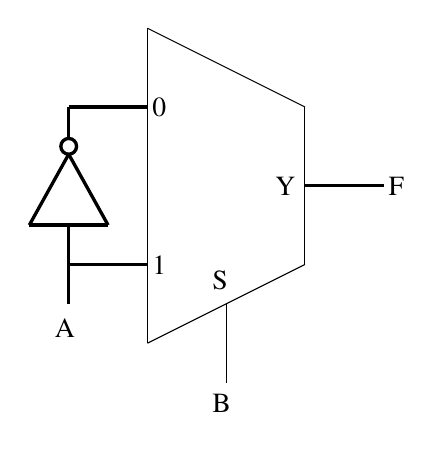
\begin{tikzpicture}
	\draw[draw=black, thin, solid] (0.00,4.00) -- (0.00,0.00);
	\draw[draw=black, thin, solid] (2.00,3.00) -- (2.00,1.00);
	\draw[draw=black, thin, solid] (0.00,0.00) -- (2.00,1.00);
	\draw[draw=black, thin, solid] (0.00,4.00) -- (2.00,3.00);
	\draw[draw=black, very thick, solid] (2.00,2.00) -- (3.00,2.00);
	\draw[draw=black, very thick, solid] (0.00,3.00) -- (-1.00,3.00);
	\draw[draw=black, very thick, solid] (0.00,1.00) -- (-1.00,1.00);
	\draw[draw=black, thin, solid] (1.00,0.50) -- (1.00,-0.50);
	\draw[draw=black, very thick, solid] (-1.00,3.00) -- (-1.00,2.60);
	\draw[draw=black, very thick, solid] (-1.00,1.00) -- (-1.00,1.50);
	\draw[draw=black, very thick, solid] (-1.00,2.50) circle (0.1);
	\draw[draw=black, very thick, solid] (-1.00,2.40) -- (-0.50,1.50);
	\draw[draw=black, very thick, solid] (-1.00,2.40) -- (-1.50,1.50);
	\draw[draw=black, very thick, solid] (-1.50,1.50) -- (-0.50,1.50);
	\draw[draw=black, very thick, solid] (-1.00,1.00) -- (-1.00,0.50);

	\node[black, anchor=south west] at (2.94,1.75) {F
};
	\node[black, anchor=south west] at (0.70,-1) {B
};
	\node[black, anchor=south west] at (-1.30,-0.05) {A
};
	\node[black, anchor=south west] at (0.70,0.55) {S
};
	\node[black, anchor=south west] at (-0.06,2.75) {0
};
	\node[black, anchor=south west] at (-0.06,0.75) {1
};
	\node[black, anchor=south west] at (1.50,1.75) {Y
};
\end{tikzpicture}

			      \caption{}
		      \end{center}
	      \end{figure}
\begin{enumerate}
\item A $\oplus$ B \vspace{3pt}
\item $\overline{\text{A + B}}$ \vspace{3pt}
\item A + B \vspace{3pt}
\item  $\overline{\text{A $\oplus$ B}}$ \vspace{3pt}
\end{enumerate}
\end{enumerate}



\end{document}
